\section{State of art} 
\label{sec:state_of_art}
This section introduces a description and classification of works aiming to address the energy problem generated by employing sensors continuously in mobile sensing apps.
A special focus is given to the pure software techniques, which will be pursued during the development of this research.

\subsection{Approaches for addressing the energy issue}

As stated, the advances produced in several technological fields have contributed to the acceptance of tke smart devices, like the smartphone, by society \cite{Lane2010,Ra2012}.
However, although computing and storage capacity issues have been partially addressed and solved with every new generation of mobile devices, the energy consumption is still an open issue because of the slow rhythm of the technological advances related to it and because the inclusion of newer and more sophisticated sensors that impose a higher energy demand.

In this sense, the battery consumption concern has been under research since the introduction of mobile devices into the market, and also shows an evolution in the objectives pursued by scientists. 

The research in energy management in mobile devices started with broad techniques and guidelines applied when building mobile application systems.
In \cite{Mayo2004} the authors address the energy consumption issue from a design point of view by introducing the idea of the \emph{requirements-aware energy scale-down} approach. 

This approach states that both hardware and software elements should scale their features and energy usage to meet a variety of design points.
According to it, if there are no hard energy constraints, the software can use the hardware components at maximum performance in order to accomplish the mobile app requirements.
On the other hand, in case of energy constraints the mobile app must be aware and react accordingly by modifying --- via software --- the hardware usage for consuming less energy and still accomplish the application requirements.
The described work was implemented targeting different hardware elements like screen, processor and wireless radio communication interfaces.
For example, the screen implementation aims the design of energy aware GUI's.
Such GUI's change the luminescence and color of non-active portions of the screen to reduce power consumption, as shown in the Figure \ref{fig-scaling-down-screen-usage}.

\begin{figure}
        \centering
        \begin{subfigure}[b]{0.3\textwidth}
                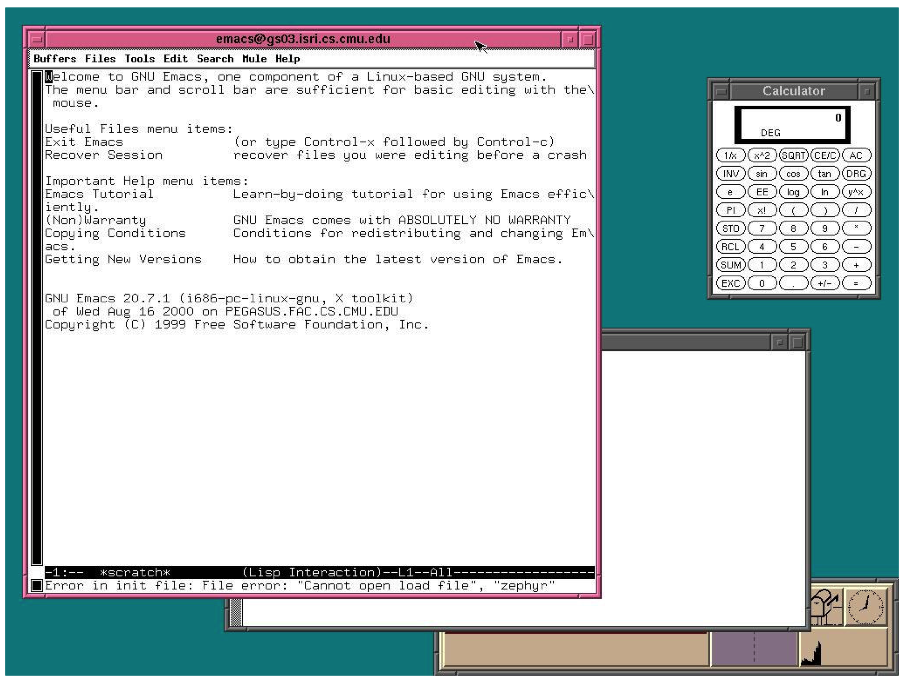
\includegraphics[width=\textwidth]{energy-aware-gui-1}
                \caption{Original interface}
                \label{fig:energy-aware-gui-1}
        \end{subfigure}
        ~
        \begin{subfigure}[b]{0.3\textwidth}
                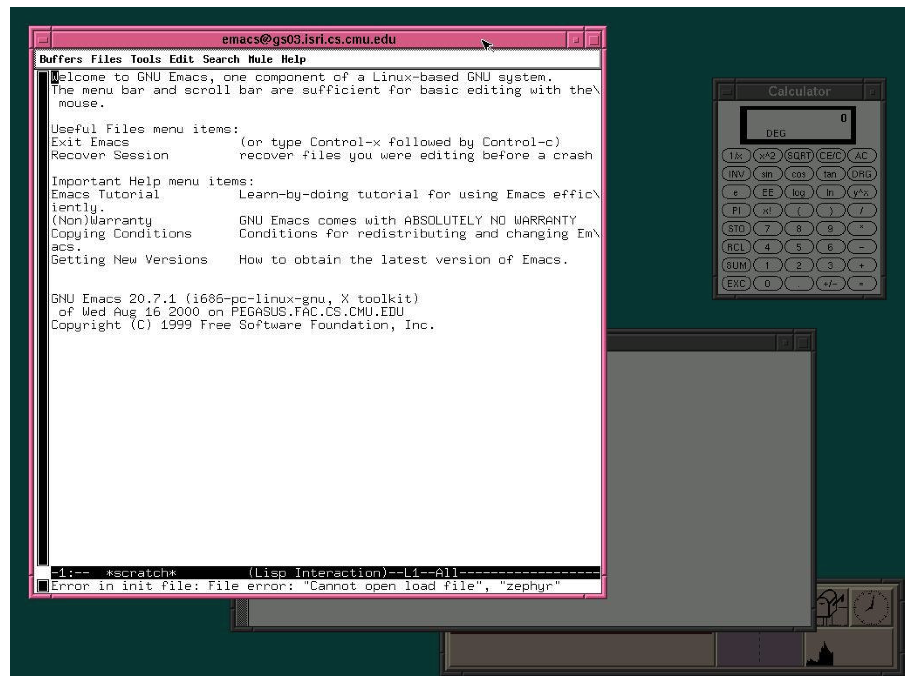
\includegraphics[width=\textwidth]{energy-aware-gui-2}
                \caption{Background half dim}
                \label{fig:energy-aware-gui-2}
        \end{subfigure}
        ~
        \begin{subfigure}[b]{0.3\textwidth}
                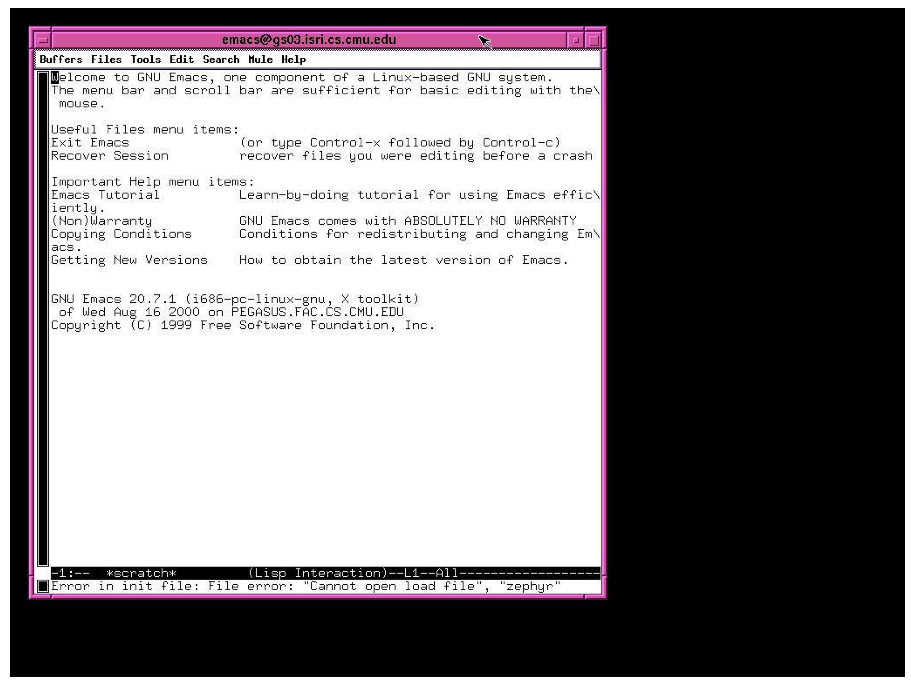
\includegraphics[width=\textwidth]{energy-aware-gui-3}
                \caption{Background fully dim}
                \label{fig:energy-aware-gui-3}
        \end{subfigure}
        \caption[An example of energy aware GUI by \protect\cite{Mayo2004}]{An example of energy aware GUI proposed by \protect\cite{Mayo2004}}
        \label{fig-scaling-down-screen-usage}
\end{figure}

The idea of \emph{requirements-aware energy scale-down} approach serves as a base for the creation of specific techniques for addressing the energy consumption issue.
However, the work introduced by authors focused on broad guidelines that, while helpful, left behind important details that can be obtained from contextual information of user.
It is noteworthy that at the time of the coinage of this approach the smart devices proliferation was in its infancy.

Currently, the popularity of smartphones and the mobile sensing apps have made the energy issue evident and specific mechanisms have been proposed to address it.
A revision of the literature shows that there are three families of techniques to face the energy issue (Figure \ref{fig:approaches-taxonomy}): 

\begin{itemize}
  \item Pure hardware.
  \item Hardware-software.
  \item Pure software.
\end{itemize}

The pure-hardware approach is located at hardware level and is agnostic of the entire software platform.
The hardware-software approach is located at the lowest levels of the mobile OS in connection with hardware elements.
It can be seen as the development of new hardware drivers.
Finally, the pure-software approach is located at top of the mobile OS stack and it is agnostic of the hardware platform.
Works of this approach make use of the API offered by the mobile OS for accessing sensors, collect data, analyze these data and readapt the usage of sensors.

\begin{figure}
\centering
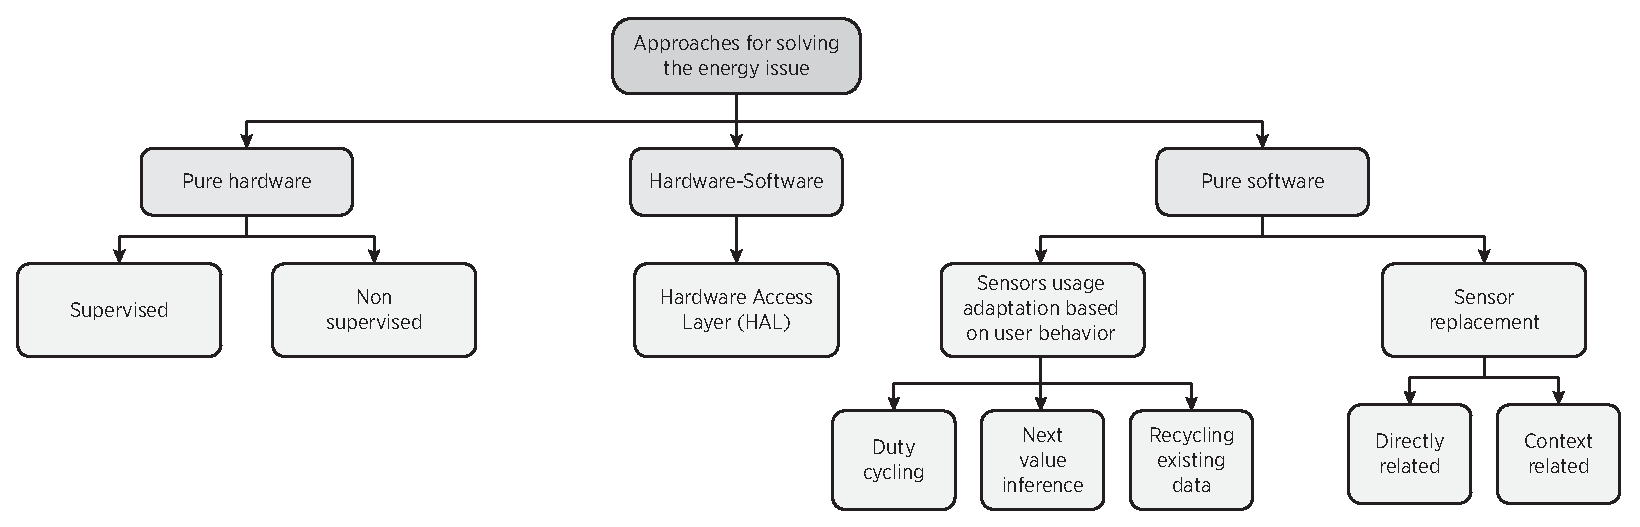
\includegraphics[width=\textwidth]{approaches-taxonomy}
\caption[Taxonomy of approaches for solving the energy issue]{Taxonomy of approaches for solving the energy issue.}
\label{fig:approaches-taxonomy}
\end{figure}

As can be seen in Figure \ref{fig:cross-layer-approaches}, the energy issue is a cross-layer problem that can be analyzed and addressed from several perspectives.
It is noteworthy that although there is a taxonomy of approaches, the solutions found in literature may include a combination of these techniques.
This is a suggestion of the complexity of the problem and even about the evolution of the techniques, since ideas proved to be working efficiently in software soon or later are implemented directly in hardware. 
\begin{figure}
\centering
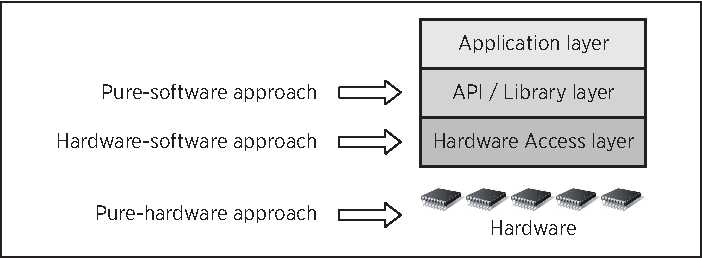
\includegraphics[scale=0.7]{cross-layer-approaches}
\caption[Energy issue as an OS cross-platform problem]{The relation between approaches for solving the energy issue and layers of a mobile platform.}
\label{fig:cross-layer-approaches}
\end{figure}

The Figure \ref{fig:approaches-description} shows how the different approaches are materialized in the hardware platform. Note that the pure hardware approach modifies directly the frequency and voltage introduced to the hardware circuits, defining the power states of the components.

In the same figure, it can be seen that the hardware-software approach defines periods to keep the same sensor turned on or off, building a \emph{hardware access layer} above the bolts and nuts of the platform.

Finally, the same figure shows that the pure software approach tries to define an even higher layer for modifying the behavior of the different sensors present in the mobile platform. The duty cycling of different sensors can be manipulated in order to obtain high level information --- meaningful for user --- and at the same time lowering the impact on battery.

The Table \ref{fig:tabla} shows a set of works found in the literature that aim to solve the energy issue in mobile sensing apps.
An important aspect of these works is that because of their differences in approaches and purpose, a direct comparison is not possible to perform \cite{Vallina-Rodriguez2013}.
\begin{figure}
\centering

\includegraphics[scale=1.2]{tabla}
\caption[Works aiming to solve the energy issue in MSA]{Set of works aiming to solve the energy issue in mobile sensing apps.}
\label{fig:tabla}
\end{figure}


In next sections a brief description of the pure hardware and hardware-software approaches is presented, followed by a detailed review of the pure software approach since the special features and advantages offered by it.
Inside each description some of the works presented in the Table \ref{fig:tabla} are also reviewed.

\begin{figure}
\centering
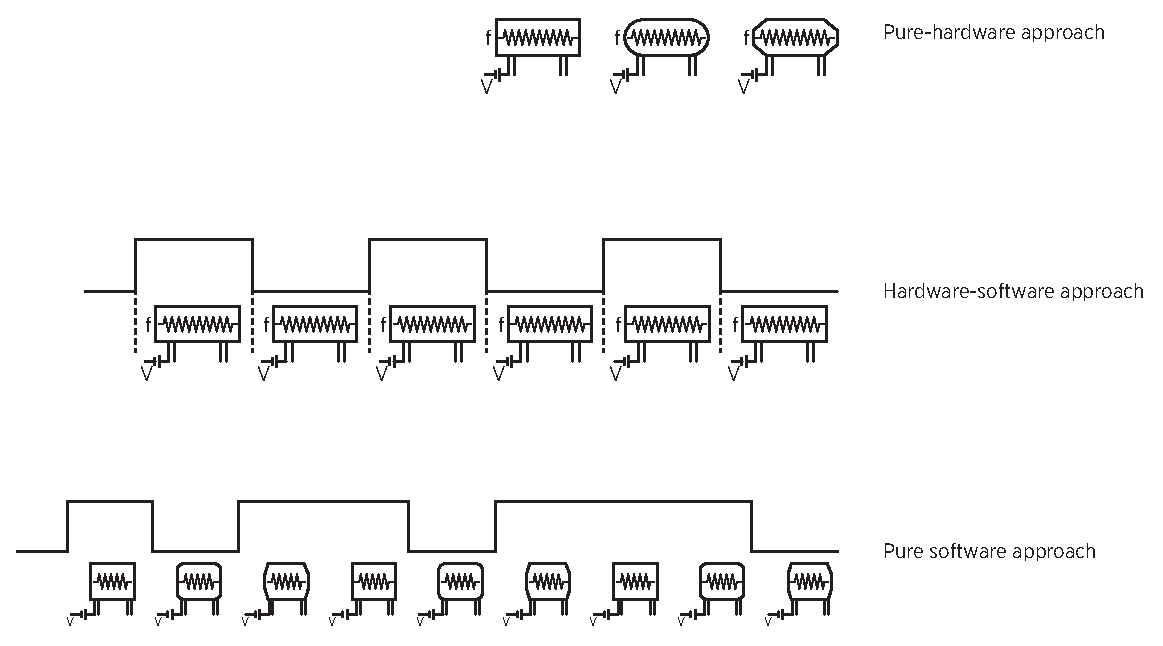
\includegraphics[scale=0.7]{approaches-description}
\caption[Approaches seen from hardware perspective]{The approaches seen from a hardware perspective.}
\label{fig:approaches-description}
\end{figure}

\subsubsection{Pure hardware approach}

Despite the fact current mobile processors include features at the electronic level like DPM\footnote{DPM, Dynamic Power Management} and DVFS\footnote{DVFS, Dynamic Voltage and Frequency Scaling} that are helpful to reduce the energy consumed by them, these techniques are not enough to solve the energy issue in mobile platforms.
The major drawback with the usage of these features is the complexity of the mobile processors, whose static power consumption remains high (approximately 200mW) when the processor is not in sleep mode \cite{Priyantha2011}.
Additionally, the current architecture of most mobile platforms require that for the correct operation of the phone, other components have to be operational, which increases the energy consumption.

This approach is focused in adapting physical features of hardware components in order to reduce the energy consumption.
The most used physical features are the frequency and voltage introduced to the hardware elements.
In this way, the hardware designers define and introduce the different operational states of the physical components of the platform.

Works under this approach typically involve a hardware rearrangement to exploit the previously mentioned features.
This redesign implies the isolation of all of the components associated with the measurement of physical signals inside a new unit with a dedicated low power processor.
Such change must not carry a modification inside the mobile apps' logic.

This new hardware unit can obtain a substantial reduction in the energy consumption since it is energy aware by design.
The basic behavior involves that the sensors report their readings to the embedded low power processor, which is capable of doing light computing operations like filtering.
While the hardware unit is working on reading and filtering data, the rest of the smartphone's hardware platform is able to reach its sleep mode.

The pure hardware approach can be materialized following two distinct implementations, based on the level of data complexity that the platform can handle.

\subparagraph{Not autonomous variant}
\label{subp:not_autonomous_variant}

The \textbf{not autonomous} does not have knowledge about the information that is handled and it is restricted to receive sensor data requests and deliver data without running any sort of filtering or processing.

An example of the not autonomous variant is LittleRock \cite{Priyantha2011}.
Its design includes a special unit in charge of the access to sensors.
When any mobile app requires to perform sensing tasks it has the option to employ the LittleRock unit or use it only as a bridge and access directly to sensors.
The relevant features of this design are:

\begin{description}
  \item[Power independence] LittleRock is powered directly from battery and not from other internal electronic items.
  Because of this, the main circuitry can be turned off when the phone is in sleep mode and keep LittleRock accessing to sensors.
  
  \item[Interrupt] LittleRock offers interruption features, making it possible to wake up the phone and inform it about events discovered in data delivered by sensors.
  
  \item[Re-purposing] LittleRock allows to reprogram its main processor to adapt the processing of sensor data and achieve mobile app requirements.
\end{description}

The experimentation conducted by authors indicates that LittleRock can operate up to 830 days whe this and the phone are in sleep mode using a 1340 mAH battery.
Among the results, it is noteworthy that LittleRock is faster than the phone itself do collect a single sample of data from sensors due to the complexity of the software stack that the main processor has to handle.

Another relevant example of the supervised variant is reported in \cite{Choudhury2008}.
Despite the fact this work was not implemented in a smartphone unit, it also introduces a mobile sensing platform (MSP) that is composed in a similar way than LittleRock.
This MSP is basically a sensor board attached to a wireless node that includes a 32 bits ARM7 processor, Bluetooth interface and a compact flash bay for storage.
It can be noted that the MSP is representing the extra hardware unit with sensors and a dedicated low power processor, which can deliver the collected data via Bluetooth to an external computing unit for analysis and classification tasks.


\subparagraph{Autonomous variant}
\label{subp:autonomous_variant}

The \textbf{autonomous variant} is also able to deliver raw data, but additionally can detect higher level information thanks to the data processing algorithms.
For example, it might measure the distance covered by user, the amount of steps done, or identify the type of activity performed by the user (no movement, walking, running, etc.) completely by itself.


The autonomous variant has been already implemented in the Apple iPhone.
Starting from the iPhone 5s model, this smartphones family includes an ARM coprocessor that is in charge of interacting with several sensors like accelerometer, gyroscope and magnetometer in order to obtain data about user's fitness \cite{Sathiah2013}.

Apple has introduced a software API into the iPhone OS, the Core Motion Framework \cite{Apple2013}, that allows mobile app developers to make use of the new hardware architecture and to access and consume this information.
The Core Motion Framework is able to deliver information refering to amount of steps or distance that user has covered and even the type of activity performed by him.
Additionally, this API allows requests for raw data from sensors being the update frequency the only mandatory argument.

Despite the fact this implementation will lead to energy savings, it presents two major drawbacks.
The first one is that the step counter mechanism is always running in the background even if no applications are requesting data.
The second one is that this implementation does not provide support for continuous readings and lacks the idea of self adapting the sensor's duty cycle in order to reduce energy consumption.

A common problem of any hardware approach resides in that hardware designers can not foresee the needs of any future mobile development and implement them directly in the circuits.
In this sense, the effort of hardware designers is affected by a trade off between the features provided out-of-the box and the flexibility features offered by the produced hardware platform.

\subsubsection{Hardware-software approach}

Another approach found in literature describes a combination of hardware and software techniques to optimize the energy consumption in continuous sensing mobile apps.

This approach leverages physical information about sensors and basic data from context information in order to create basic rules to decide the best moment for turning sensors on and off.

% This technique aims to contribute with a reviewed and improved software API that allows to allocate computational and sensing tasks in components others than the predefined by the platform's original design.

By knowing the hardware platform, it is possible to change the behavior of the elements and employ them in a different manner.
An example of this idea is to enable an additional low power processor in the smartphone to execute any arbitrary instruction instead of the main processor.
Since the smartphone's processor can be kept idle there is a potential energy saving.

The work presented in \cite{Ra2012} leverages the presence of several low power processors (LP) in the latest smartphones.
The utilization of these LP's can be done by exposing their functionality through a layered API.

Through several simulations, authors show that such processors can bring substantial energy savings, specially when executing frequent sampling \& buffering and basic arithmetic operations.

That work describes two main challenges, the selection of a suitable LP and guidelines for deciding where to allocate the execution of a given task.
To select an adequate LP, the key factor is the wake up transition delay in terms of energy. So, any processor with a small wakeup transition delay is suitable as LP.
For deciding where to perform the execution of a task, the next guidelines are proposed:
\begin{description}
  \item[Execution in main processor]{Tasks found to be more efficient in the main processor should be executed there, ignoring the transition penalty}.
  \item[Execution in LP]{Tasks found to be more efficient in the LP, and that are very frequent within the mobile app, should be executed in the LP. Sampling and buffering tasks belong to this category}.
  \item[Execution in main or in LP]{Tasks found to be more efficient in the LP, and  that are not frequent within the mobile app, should be executed in the LP. However, a special mechanism to evict them should be included. This might happen when tasks of other mobile apps request the LP}.
\end{description}
